% ----------------------------------------------------------
% Capítulo 1
% ----------------------------------------------------------
\chapter{Arquitetura do Sistema - Diagrama C4}
\label{chap:arquitetura-c4}

Para ilustrar claramente a arquitetura proposta para o Sistema VOEBEM, utilizamos a metodologia C4 Model. Esta abordagem fornece diferentes níveis de detalhe, desde uma visão geral do contexto até a estrutura interna dos componentes principais, facilitando a compreensão por diferentes públicos (técnicos e de negócio).

\section{Nível 1 (Contexto)}
\label{sec:c4-contexto}

Este diagrama mostra o Sistema de Reservas VOEBEM em seu contexto, identificando os principais usuários e as integrações com sistemas externos essenciais para sua operação.

\begin{figure}[htbp]
    \centering
    % Nota: A compilação de SVG pode exigir pacotes adicionais como 'svg'.
    % Considere converter as imagens para PDF ou pdf para compatibilidade padrão com pdflatex.
    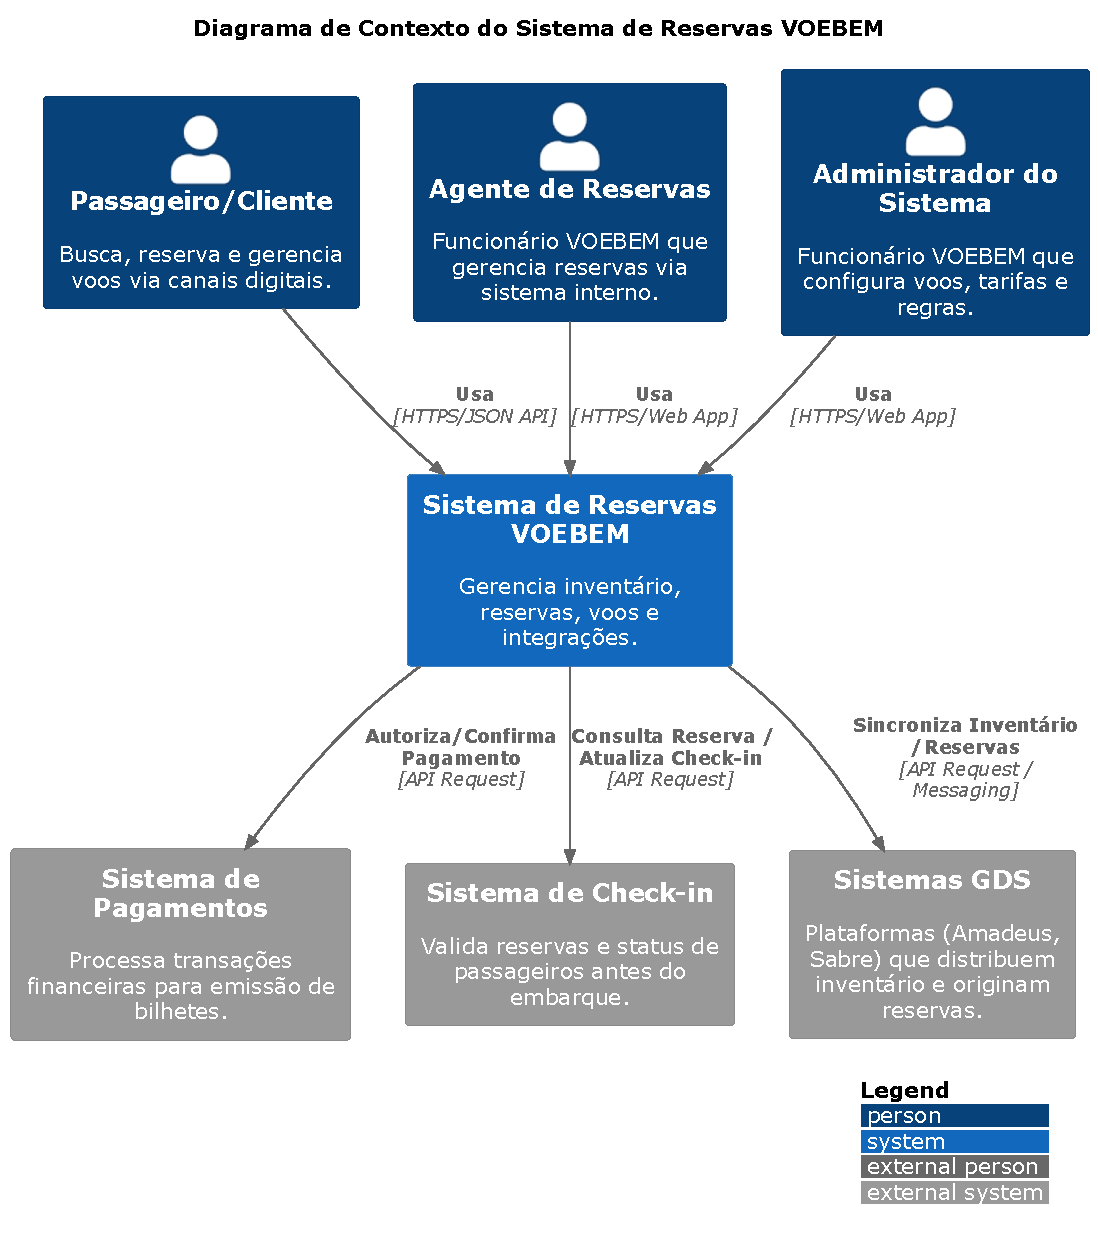
\includegraphics[width=0.9\textwidth]{c4-n1-contexto.pdf}
    \caption{Diagrama de Contexto C4 - Sistema VOEBEM}
    \label{fig:c4-contexto}
\end{figure}

\subsection{Usuários (Personas)}
\label{subsec:c4-contexto-usuarios}
\begin{itemize}
    \item \textbf{Passageiro/Cliente:} Pessoa que busca, reserva e gerencia voos através dos canais digitais (Website/App Mobile).
    \item \textbf{Agente de Reservas (Funcionário VOEBEM):} Funcionário que utiliza o sistema internamente para criar, modificar e gerenciar reservas em nome dos clientes.
    \item \textbf{Administrador do Sistema (Funcionário VOEBEM):} Funcionário responsável pela configuração de voos, tarifas, regras de negócio e gerenciamento geral do sistema.
\end{itemize}

\subsection{Sistema Principal}
\label{subsec:c4-contexto-sistema-principal}
\begin{itemize}
    \item \textbf{Sistema de Reservas VOEBEM (Software System):} A aplicação central que gerencia todo o inventário de voos, trechos, assentos, processa reservas e fornece informações aos usuários e sistemas externos.
\end{itemize}

\subsection{Sistemas Externos}
\label{subsec:c4-contexto-sistemas-externos}
\begin{itemize}
    \item \textbf{Sistema de Pagamentos (External System):} Serviço externo responsável pelo processamento seguro de transações financeiras para a emissão de bilhetes. \textit{Interage com o Sistema VOEBEM para autorizar e confirmar pagamentos.}
    \item \textbf{Sistema de Check-in (External System):} Sistema utilizado nos aeroportos (ou online) para validar reservas, confirmar a presença do passageiro e atribuir/confirmar assentos antes do embarque. \textit{Interage com o Sistema VOEBEM para consultar dados da reserva/assento e atualizar o status de check-in.}
    \item \textbf{Sistemas GDS (Global Distribution Systems) (External System):} Plataformas globais (Exemplo: Amadeus, Sabre) que distribuem o inventário de voos da VOEBEM para agências de viagens e outros canais. \textit{Interage com o Sistema VOEBEM para consultar disponibilidade, criar reservas (originadas externamente) e sincronizar informações.}
\end{itemize}

\section{Nível 2 (Container)}
\label{sec:c4-container}

Este diagrama detalha os principais blocos de construção (containers) do Sistema de Reservas VOEBEM, suas responsabilidades, tecnologias e como eles interagem, utilizando um banco de dados centralizado conforme requisito.

\begin{figure}[htbp]
    \centering
    % Ajustando largura para consistência com Cap. 3
    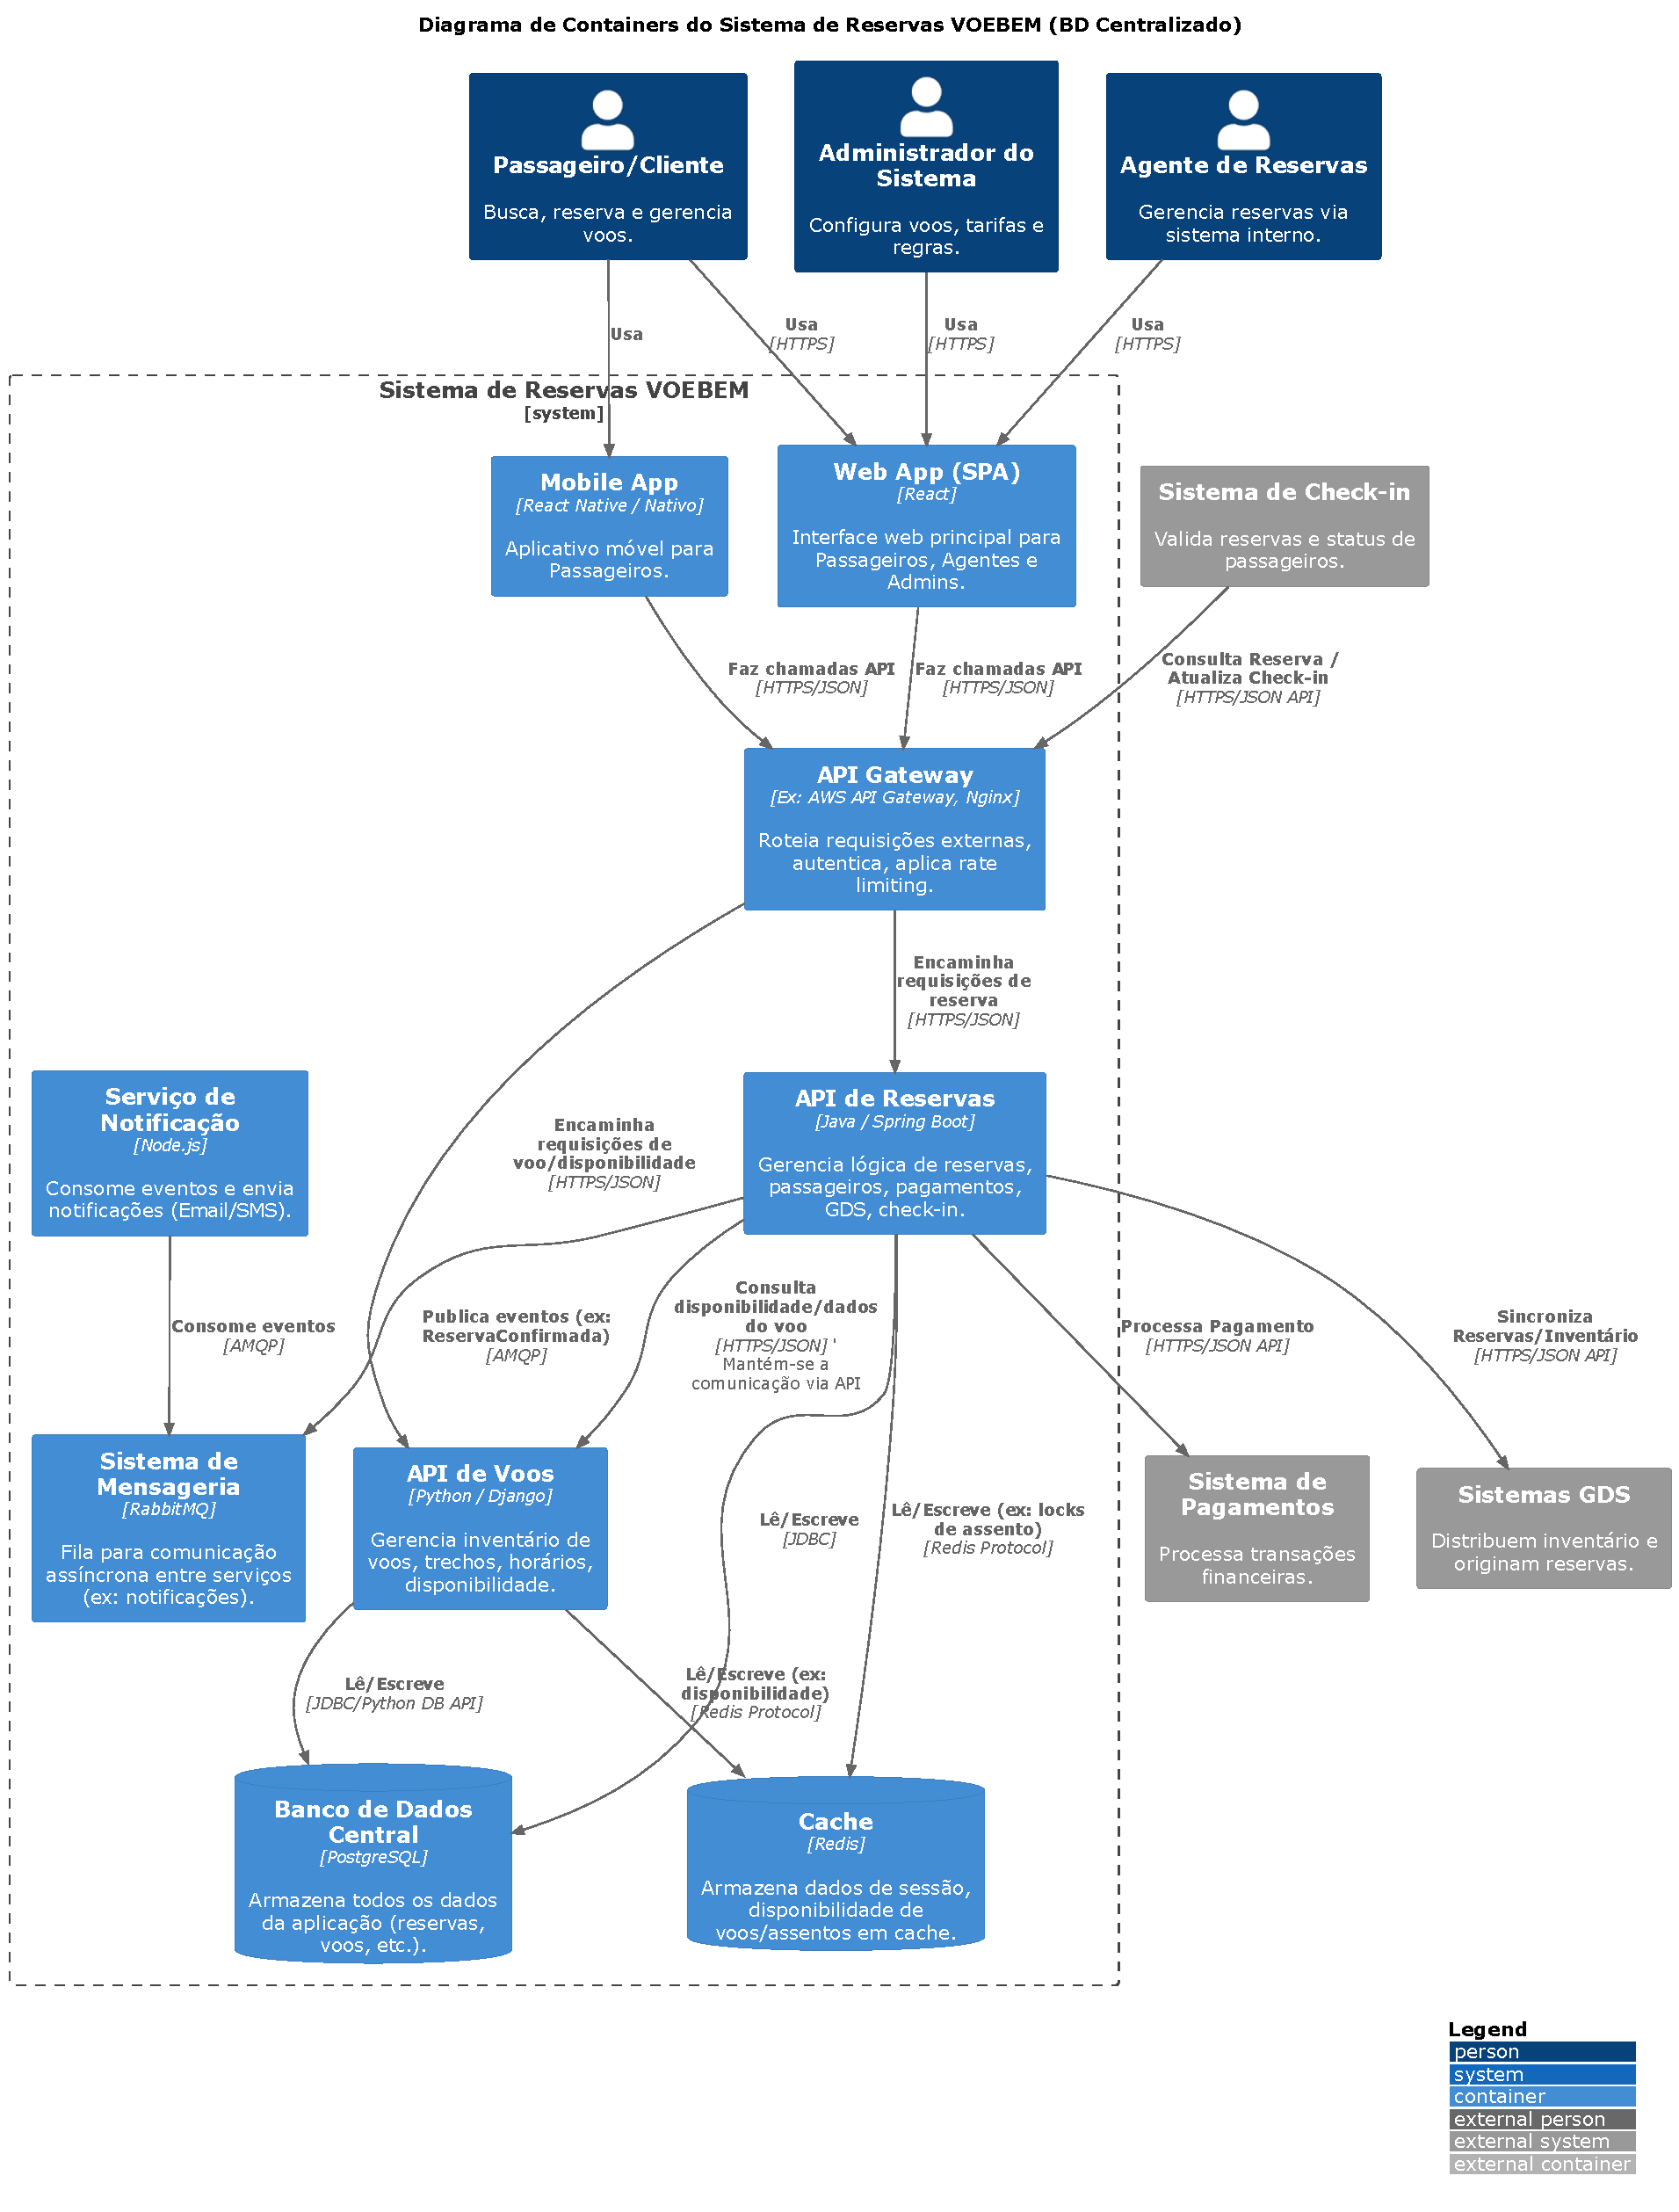
\includegraphics[width=0.8\textwidth]{c4-n2-container.pdf}
    \caption{Diagrama de Containers C4 - Sistema VOEBEM}
    \label{fig:c4-container}
\end{figure}

\subsection{Containers Principais}
\label{subsec:c4-container-principais}

\textbf{Web App (SPA) (Container)}
\begin{itemize}
    \item \textbf{Descrição:} Interface web principal acessada via navegador.
    \item \textbf{Tecnologia:} React.
    \item \textbf{Responsabilidade:} Fornecer a interface do usuário para Passageiros, Agentes de Reservas e Administradores realizarem suas tarefas (consultas, reservas, gerenciamento).
    \item \textbf{Interage com:} API Gateway (via HTTPS/JSON).
\end{itemize}

\textbf{Mobile App (Container)}
\begin{itemize}
    \item \textbf{Descrição:} Aplicativo móvel nativo ou híbrido.
    \item \textbf{Tecnologia:} React Native / Nativo (iOS/Android).
    \item \textbf{Responsabilidade:} Fornecer uma interface otimizada para Passageiros em dispositivos móveis.
    \item \textbf{Interage com:} API Gateway (via HTTPS/JSON).
\end{itemize}

\textbf{API Gateway (Container)}
\begin{itemize}
    \item \textbf{Descrição:} Ponto único de entrada para todas as requisições externas das interfaces (SPA, Mobile App) e de sistemas externos (Check-in).
    \item \textbf{Tecnologia:} Exemplo: AWS API Gateway, Nginx, Kong.
    \item \textbf{Responsabilidade:} Roteamento de requisições para os serviços backend apropriados, autenticação/autorização inicial, aplicação de rate limiting, agregação leve de respostas (opcional).
    \item \textbf{Interage com:} Web App, Mobile App, Sistema de Check-in, API de Reservas, API de Voos.
\end{itemize}

\textbf{API de Reservas (Container)}
\begin{itemize}
    \item \textbf{Descrição:} Microsserviço backend focado no domínio de reservas.
    \item \textbf{Tecnologia:} Java / Spring Boot.
    \item \textbf{Responsabilidade:} Gerenciar todo o ciclo de vida das reservas (criação, consulta, cancelamento, prorrogação), dados de passageiros, orquestrar interações com pagamento, GDS e check-in, gerenciar reserva de assentos.
    \item \textbf{Interage com:} API Gateway, Banco de Dados Central, API de Voos, Cache, Sistema de Mensageria, Sistema de Pagamentos, Sistemas GDS.
\end{itemize}

\textbf{API de Voos (Container)}
\begin{itemize}
    \item \textbf{Descrição:} Microsserviço backend focado no domínio de inventário de voos.
    \item \textbf{Tecnologia:} Python / Django.
    \item \textbf{Responsabilidade:} Gerenciar informações sobre voos, trechos, horários, aeroportos, aeronaves e calcular/consultar disponibilidade de voos e assentos.
    \item \textbf{Interage com:} API Gateway, Banco de Dados Central, Cache, API de Reservas.
\end{itemize}

\textbf{Serviço de Notificação (Container)}
\begin{itemize}
    \item \textbf{Descrição:} Serviço assíncrono para envio de notificações.
    \item \textbf{Tecnologia:} Node.js.
    \item \textbf{Responsabilidade:} Consumir eventos do Sistema de Mensageria (Exemplo: \texttt{ReservaConfirmada}, \texttt{PrazoExpirando}) e enviar notificações aos usuários via canais apropriados (Email, SMS - integração com serviços externos específicos não mostrada neste nível).
    \item \textbf{Interage com:} Sistema de Mensageria.
\end{itemize}

\subsection{Containers de Dados e Mensageria}
\label{subsec:c4-container-dados}

\textbf{Banco de Dados Central (Database Container)}
\begin{itemize}
    \item \textbf{Descrição:} Banco de dados relacional centralizado que armazena todos os dados da aplicação.
    \item \textbf{Tecnologia:} PostgreSQL.
    \item \textbf{Responsabilidade:} Armazenar de forma persistente e transacional os dados de reservas, passageiros, voos, trechos, aeroportos, aeronaves, assentos, etc.
    \item \textbf{Acessado por:} API de Reservas, API de Voos.
\end{itemize}

\textbf{Cache (Database Container)}
\begin{itemize}
    \item \textbf{Descrição:} Armazenamento de dados em memória para acesso rápido.
    \item \textbf{Tecnologia:} Redis.
    \item \item \textbf{Responsabilidade:} Acelerar consultas frequentes (Exemplo: disponibilidade de voos/assentos), armazenar dados de sessão (opcional), gerenciar locks temporários (Exemplo: durante seleção de assento).
    \item \textbf{Acessado por:} API de Reservas, API de Voos.
\end{itemize}

\textbf{Sistema de Mensageria (Container)}
\begin{itemize}
    \item \textbf{Descrição:} Broker de mensagens para comunicação assíncrona.
    \item \textbf{Tecnologia:} RabbitMQ.
    \item \textbf{Responsabilidade:} Desacoplar a comunicação entre serviços, permitindo que eventos sejam publicados (pela API de Reservas) e consumidos (pelo Serviço de Notificação) de forma independente e resiliente.
    \item \textbf{Acessado por:} API de Reservas, Serviço de Notificação.
\end{itemize}

\section{Nível 3 (Componentes - Exemplo para API de Reservas)}
\label{sec:c4-componentes}

Este diagrama detalha a estrutura interna do container "API de Reservas", mostrando seus principais componentes lógicos e como eles colaboram para realizar as funcionalidades de reserva e interagir com dependências externas.

\begin{figure}[htbp]
    \centering
    % Adicionando angle=90 para rotacionar a imagem
    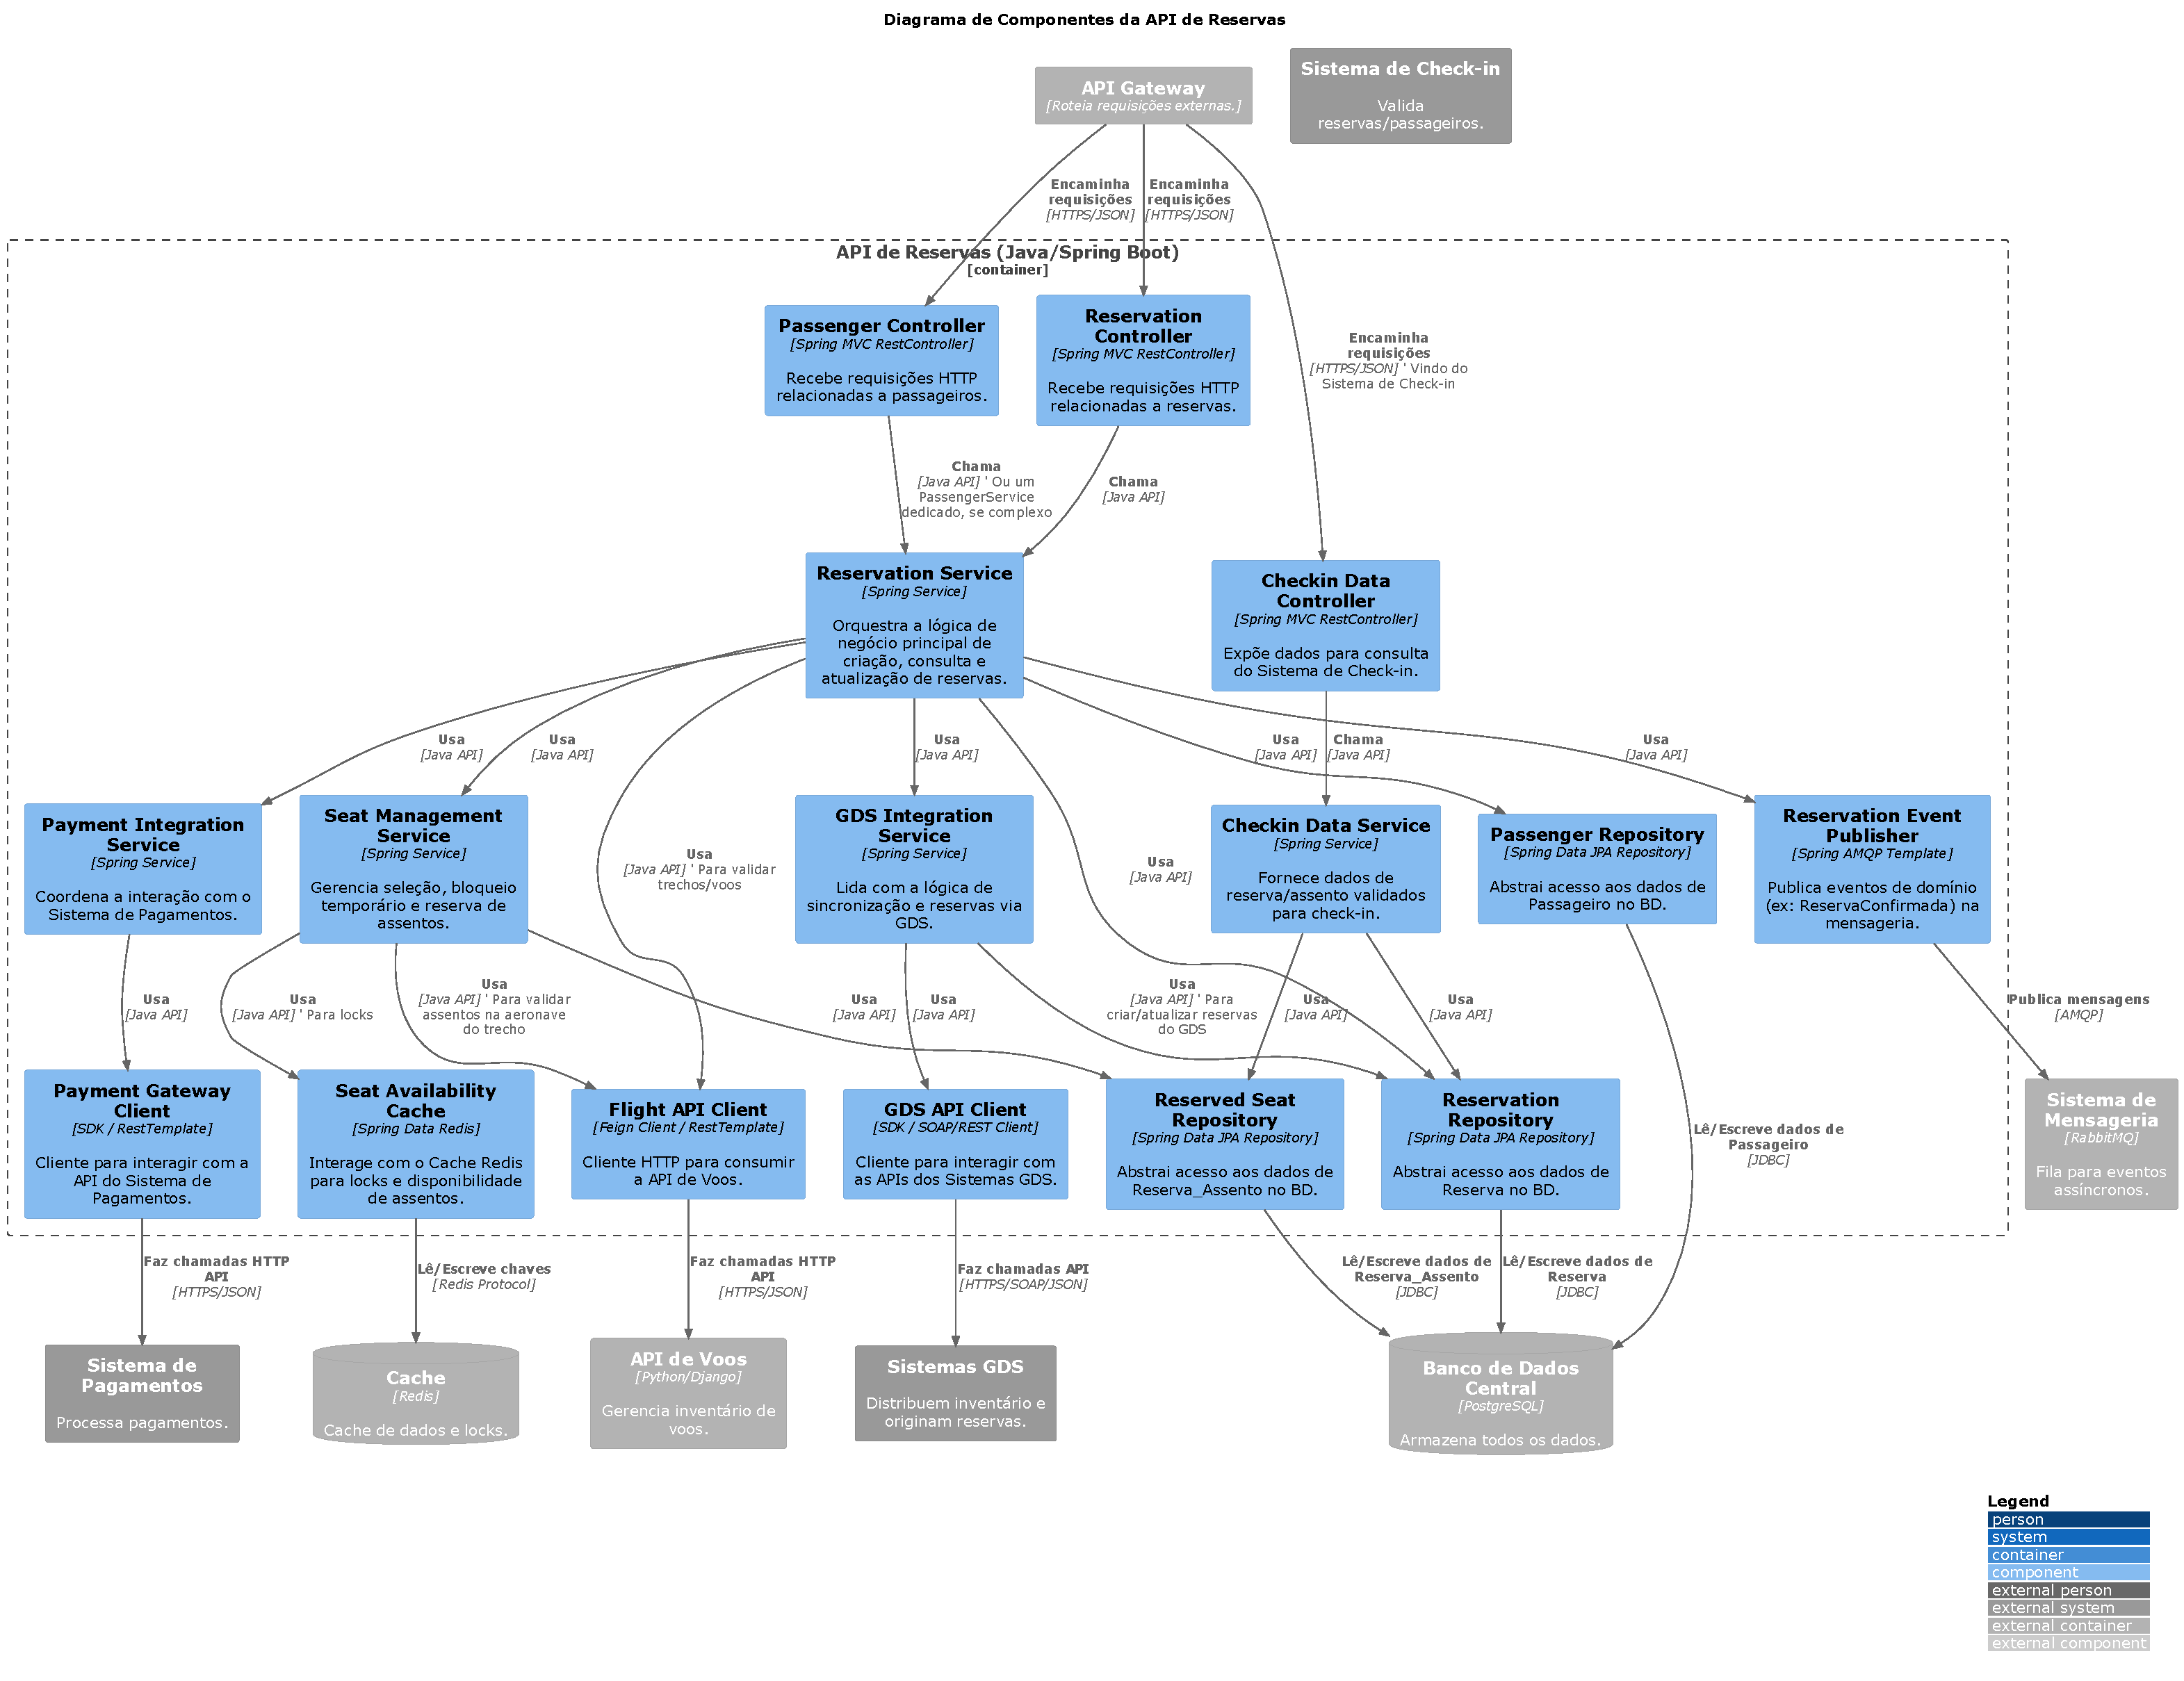
\includegraphics[width=1.4\textwidth, angle=90]{c4-n3-component-api-reservas.pdf}
    \caption{Diagrama de Componentes C4 - API de Reservas}
    \label{fig:c4-componentes-api-reservas}
\end{figure}

\subsection{Componentes Principais da API de Reservas}
\label{subsec:c4-componentes-api-reservas-principais}

\textbf{Controllers (\texttt{ReservationController}, \texttt{PassengerController}, \texttt{CheckinDataController})}
\begin{itemize}
    \item \textbf{Tecnologia:} Spring MVC RestController.
    \item \textbf{Responsabilidade:} Receber requisições HTTP da API Gateway, validar entradas básicas e delegar para os serviços apropriados. O \texttt{CheckinDataController} expõe endpoints específicos para consulta pelo Sistema de Check-in.
\end{itemize}

\textbf{Services (\texttt{ReservationService}, \texttt{SeatManagementService}, \texttt{PaymentIntegrationService}, \texttt{GdsIntegrationService}, \texttt{CheckinDataService})}
\begin{itemize}
    \item \textbf{Tecnologia:} Spring Service.
    \item \textbf{Responsabilidade:} Contêm a lógica de negócio principal.
    \begin{itemize}
        \item \texttt{ReservationService}: Orquestra o fluxo de criação, consulta, atualização de reservas, validações de regras de negócio.
        \item \texttt{SeatManagementService}: Gerencia a lógica de seleção, bloqueio temporário (usando cache) e confirmação de assentos.
        \item \texttt{PaymentIntegrationService}: Coordena a comunicação com o \texttt{PaymentGatewayClient} para processar pagamentos.
        \item \texttt{GdsIntegrationService}: Lida com a lógica de receber/enviar dados de/para os \texttt{Sistemas GDS} através do \texttt{GdsApiClient}.
        \item \texttt{CheckinDataService}: Fornece dados consolidados e validados sobre a reserva e assento para o \texttt{CheckinDataController}.
    \end{itemize}
\end{itemize}

\textbf{Repositories (\texttt{ReservationRepository}, \texttt{PassengerRepository}, \texttt{ReservedSeatRepository})}
\begin{itemize}
    \item \textbf{Tecnologia:} Spring Data JPA Repository.
    \item \textbf{Responsabilidade:} Abstrair o acesso (leitura/escrita) aos dados das entidades correspondentes no \texttt{Banco de Dados Central}.
\end{itemize}

\textbf{Clients (\texttt{FlightApiClient}, \texttt{PaymentGatewayClient}, \texttt{GdsApiClient})}
\begin{itemize}
    \item \textbf{Tecnologia:} Feign Client / RestTemplate / SDKs específicos.
    \item \textbf{Responsabilidade:} Encapsular a comunicação via rede com outros containers ou sistemas externos.
    \begin{itemize}
        \item \texttt{FlightApiClient}: Comunica-se com a \texttt{API de Voos} para obter informações de voos, trechos e validar disponibilidade/assentos.
        \item \texttt{PaymentGatewayClient}: Interage com o \texttt{Sistema de Pagamentos} externo.
        \item \texttt{GdsApiClient}: Interage com os \texttt{Sistemas GDS} externos.
    \end{itemize}
\end{itemize}

\textbf{Messaging (\texttt{ReservationEventPublisher})}
\begin{itemize}
    \item \textbf{Tecnologia:} Spring AMQP Template.
    \item \textbf{Responsabilidade:} Publicar eventos de domínio significativos (Exemplo: \texttt{ReservaConfirmada}, \texttt{PagamentoFalhou}) no \texttt{Sistema de Mensageria} para processamento assíncrono (Exemplo: notificações).
\end{itemize}

\textbf{Caching (\texttt{SeatAvailabilityCache})}
\begin{itemize}
    \item \textbf{Tecnologia:} Spring Data Redis.
    \item \textbf{Responsabilidade:} Interagir com o \texttt{Cache (Redis)} para operações específicas, como gerenciamento de locks distribuídos durante a seleção de assentos para evitar concorrência.
\end{itemize}

\section{Destaques Obrigatórios}
\label{sec:destaques-obrigatorios}

\subsection{Escalabilidade}
\label{subsec:escalabilidade}
\begin{itemize}
    \item \textbf{Horizontal:} Utilização de múltiplos containers/instâncias para os serviços (Frontend, API Gateway, Serviços Backend) gerenciados por orquestradores (Kubernetes, AWS ECS) ou grupos de autoescalonamento (Auto Scaling Groups). O Banco de Dados pode escalar leituras com réplicas.
    \item \textbf{Vertical:} Aumento de recursos (CPU/Memória) das instâncias/containers conforme necessário (menos preferível para serviços stateless).
\end{itemize}

\subsection{Balanceamento de Carga}
\label{subsec:balanceamento-carga}
Uso de Load Balancers (Exemplo: AWS ELB, Nginx) na frente da API Gateway e dos serviços backend para distribuir o tráfego entre as instâncias disponíveis.

\subsection{Alta Disponibilidade}
\label{subsec:alta-disponibilidade}
\begin{itemize}
    \item Deploy das instâncias/containers em múltiplas Zonas de Disponibilidade (AZs) na nuvem.
    \item Uso de bancos de dados gerenciados com replicação multi-AZ e failover automático.
    \item Implementação de Health Checks para que o Load Balancer e o orquestrador removam instâncias não saudáveis.
\end{itemize}

% --- Final do Arquivo ---